\documentclass[aspectratio=169]{beamer}
\usepackage{mathtools}
\usepackage{multirow}
\usepackage{multicol}
\newcommand{\pd}[2]{\frac{\partial #1}{\partial #2}}
\newcommand{\abs}[1]{\left|#1\right|}

\begin{document}
	\frame{
		\centering
		\Huge
		One- and Two-Dimensional Poisson's Equation
		\\\vspace{1.2cm}
		\large Pierce Hunter, Nick Kuckuck, Haoran Wang
		\\\vspace{0.8cm}
		\normalsize CIS 410/510 Final Presentation
		\\ 8$ ^{\text{th}} $ June 2020
	}
	\frame{
		\frametitle{Outline}
		\begin{enumerate}
			\item One dimensional model
			\begin{itemize}
				\item Equation
				\item Discretization
				\item Matrix formulation
			\end{itemize}
			\item Two-dimensional approach
			\begin{itemize}
				\item Equation
				\item Discretization
				\item Matrix formulation
			\end{itemize}
			\item Code samples
			\item Results
			\begin{itemize}
				\item One dimensional with convergence tests
				\item Two dimensional with error analysis
			\end{itemize}
		\end{enumerate}
	}
	\frame{
		\frametitle{One dimensional model}
		We solved the 1D equation
	\begin{equation}
		\pd{^2u}{z^2} = -1; \quad 0\leq z\leq 1
	\end{equation}
	with boundary conditions
	\begin{equation}
		\pd{u}{z}\left(1\right) = 0; \quad u(0) = 0
	\end{equation}
	in the four following ways:
	\begin{itemize}
		\item Direct solve on the CPU
		\item CG on the CPU
		\item Direct solve on the GPU
		\item CG on the GPU.
	\end{itemize}
	}
	\frame{
		\frametitle{1D Discretization}
		For the one-dimensional problem we can utilize the straight-forward centered-difference discretization from class, namely
	\begin{equation}
		\frac{u_{j-1}-2u_j+u_{j+1}}{\Delta z^2} = -1 ~~\text{for}~~ 1\leq j\leq N.
	\end{equation}
	We discretize on the boundaries as well, giving the final system of equations
	\begin{equation}
		\begin{dcases}
		\frac{-2u_2 + u_3}{\Delta z^2} = -1\\
		\frac{u_{j-1}-2u_j+u_{j+1}}{\Delta z^2} = -1;& 3\leq j\leq N-1\\
		\frac{u_{N-1} - u_N}{\Delta z^2} = -1.
		\end{dcases}
	\end{equation}
	}
	\frame{
		\frametitle{Matrix formulation}
	We can represent this system of equations as a matrix ($ A $) of the form
	\begin{equation}
		A = \frac{1}{\Delta z^2}\begin{bmatrix}
		-2&1&0&\cdots&0\\
		1&-2&1&\cdots&0\\
		\vdots&\ddots&\ddots&\ddots&\vdots\\
		0&\cdots&1&-2&1\\
		0&\cdots&0&1&-1
		\end{bmatrix}
	\end{equation}
	with the $ u $-column vector and $ b $-solution vector as
	\begin{equation}
		u = \begin{bmatrix}
		u_2\\
		\vdots\\
		u_N
		\end{bmatrix} \qquad b = \begin{bmatrix}
		-1\\\vdots\\-1
		\end{bmatrix}
	\end{equation}
	such that $ Au = b $.
	}
	\frame{
		\frametitle{Two-dimensional approach}
		We then expanded the problem to two-dimensions utilizing the same techniques. In 2D eq. (1) becomes
	\begin{equation}
		\pd{^2u}{y^2} + \pd{^2u}{z^2} = -1; \quad \begin{dcases}
		0\leq y\leq 1\\
		0\leq z\leq 1
		\end{dcases}
	\end{equation}
	and we expand the boundary conditions in (2) as
	\begin{align}
		\pd{u}{y} = 0&\text{ at }y=1\\
		\pd{u}{z} = 0&\text{ at }z=1\\
		u = 0&\text{ at }y=0\vphantom{\pd{u}{y}}\\
		u = 0&\text{ at }z=0\vphantom{\pd{u}{y}}.
	\end{align}
	}
	\frame{
		\frametitle{2D Discretization}
		We transform (7) into a system of ODE's by discretizing in space\textemdash both $ y $ and $ z $\textemdash using centered difference, such that
	\begin{equation}
		\frac{u_{i-1,j} - 2u_{i,j} + u_{i+1,j}}{{\Delta y}^2} + \frac{u_{i,j-1} - 2u_{i,j} + u_{i,j+1}}{{\Delta z}^2} = -1.
	\end{equation}
	which simplifies when $ \Delta y = \Delta z $ to
	\begin{equation}
		u_{i-1,j} + u_{i,j-1} - 4u_{i,j} + u_{i+1,j} + u_{i,j+1} = -{\Delta y}^2.
	\end{equation}
	This discretization works when $ 2\leq i\leq N $ and $ 2\leq j\leq N $, but we need to solve on the boundaries, of which there are many. The boundary conditions discretize separately for the edges and corners, which expands our boundary conditions to eight separate cases
	}
	\frame{
		\frametitle{2D Matrix formulation}
		In order to convert this discretization to a matrix that can be used for a direct solve we need to define a new indexing convention. For this we calculate a global index $ k $ as
	\begin{equation}
		k = (i-2)(N-1) + (j-1).
	\end{equation}
	We can then translate our discretization into this new system, giving nine total cases. 
	}
	
	\frame{
		\frametitle{2D Matrix formulation Cont.}
		So what we end up with is an $ (N-1)^2\times(N-1)^2 $ matrix $ A $ and a solution vector $ b $ with $ (N-1)^2 $ entries. Moving across a row we start at $ (2,2) $, to increase $ j $ by one we move to the right 1 entry, to increase $ i $ by 1 we move the right $ (N-1) $ entries, such that we hit every value of $ j $ first, then move to the next $ i $.
	\newline\indent Along the diagonals of the matrix $ A $ we have $ -4 $ except in the following locations:
	\begin{itemize}
		\item rows $ \alpha(N-1) $ the diagonal entry is $ -3 $ for $ 1\leq \alpha\leq N-2 $
		\item rows $ \left(N-2\right)\left(N-1\right)+\beta $ the diagonal is $ -3 $ for $ 1\leq\beta\leq N-2 $
		\item row $ \left(N-1\right)^2 $ the diagonal is $ -2 $
	\end{itemize}
	}
	
	\frame{
	\frametitle{2D Matrix formulation Cont.}
	We also have four other sub-diagonals that will all contain ones except where noted. These represent the following location:
	\begin{itemize}
		\item $ j-1 $ which is directly below the diagonal\\
		In Julia these are the locations: \texttt{\footnotesize[2:(N-1)$^2$, 1:(N-1)$^2$-1]}\\
		Exception: the locations $ (\alpha(N-1) + 1,\alpha(N-1)) $ should be zero for $ 1\leq\alpha\leq N-2 $
		\item $ j+1 $ which is directly above the diagonal\\
		In Julia these are the locations: \texttt{\footnotesize[1:(N-1)$^2$-1, 2:(N-1)$^2$]}\\
		Exception: the locations $ (\alpha(N-1),\alpha(N-1)+1) $ should be zero for $ 1\leq\alpha\leq N-2 $
		\item $ i-1 $ which are exactly $ N-1 $ below the diagonal\\
		In Julia these are the locations: \texttt{\footnotesize[N:(N-1)$^2$, 1:(N-1)$^2$-(N-1)]}
		\item $ i+1 $ which are exactly $ N+1 $ above the diagonal\\
		In Julia these are the locations: \texttt{\footnotesize[1:(N-1)$^2$-(N-1), N:(N-1)$^2$]}
	\end{itemize}
	}
	\frame{
		\frametitle{2D Matrix formulation Cont.}
	Once $ A $ is created it is probably easier to create a column vector of length $ (N-1)^2 $ in which every location contains $ -{\Delta y}^2 $. Once a solution is found via $ u = A\backslash b $ or CG, then $ u $ can be reshaped to the correct dimensions either manually\textemdash \texttt{\footnotesize i = floor((k-1)/(N-1)) + 2}; \texttt{\footnotesize j = mod(k-1,N-1) + 2}\textemdash or via the reshape function transposed\textemdash \texttt{\footnotesize U = reshape(u,N-1,N-1)$'$}. Using reshape without the transpose puts the solution in meshgrid format (with $ y $ as the columns and $ z $ as the rows) similar to looking at a cross-section.\\

	
	}
	\frame{
		\frametitle{Code Samples}
	
	}
	\frame{
		\frametitle{One dimensional with convergence tests}
		\subsection{One-Dimensional Problem}
	Our model solves for the velocity $ u $ as a function of depth $ z $ for a semi-random nondimensional problem. We plot $ u $ on the $ x $-axis and $ z $ as the $ y $-axis below.
	\begin{center}
		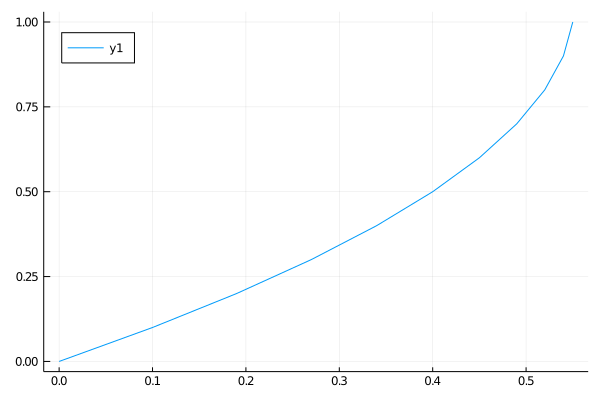
\includegraphics[scale=0.5]{1D_mid_res.png}
	\end{center}
	}
	
	\frame{
		\frametitle{1D Results}
	It is noted that velocity increases as a function of $ z $ until reaching a maximum such that the upper boundary condition is satisfied.
	\newline\indent
	We then ensured our solution was converging as expected by decreasing $ \Delta z $ by orders of 2, and checking to make sure the error was decreasing at a constant rate.
	\begin{center}
		\renewcommand{\arraystretch}{2.0}
		\begin{tabular}{c|c|c|c}
			\hline\hline
			$\displaystyle \Delta z $&$\displaystyle \varepsilon_{\Delta z} = \sqrt{z}\lVert u-e\rVert $&$ \displaystyle \Delta\varepsilon = \frac{\varepsilon_{2\Delta z}}{\varepsilon_{\Delta z}} $&$\displaystyle r = \log_2\left(\Delta\varepsilon\right) $\\
			\hline
			0.1&$3.102\times 10^{-2}$&Empty Entry&Empty Entry\\
			0.05&$1.497\times 10^{-2}$&2.072&1.051\\
			0.025&$7.352\times 10^{-3}$&2.036&1.026\\
			0.0125&$3.642\times 10^{-3}$&2.019&1.014\\
			\hline
		\end{tabular}
	\end{center}
	We do see the error decreasing linearly with decreases in $ \Delta z $, which leads us to believe we do not have instability in our system.
	\newline\indent
	}
	\frame{
		\frametitle{1D Time}
		We timed the one-dimensional problem using the four methods listed above and depict the results in the table below, keeping $ \Delta z $ constant at $ 5\times10^{-5} $ throughout.
	\begin{center}
		\renewcommand{\arraystretch}{1.5}
		\begin{tabular}{c|c|c|c}
			\hline\hline
			\textbf{Device}&\textbf{Method}&\textbf{Time [s]}&\textbf{Error~~$\sqrt{z}\lVert u-e\rVert $}\\
			\hline
			\multirow{2}{*}{CPU}&Direct&0.0426&$1.44\times 10^{-5}$\\
			&CG&15.1&$1.44\times 10^{-5}$\\
			\hline
			\multirow{2}{*}{GPU}&Direct&1.13&$1.44\times 10^{-5}$\\
			&CG&3.19&$1.44\times 10^{-5}$\\
			\hline
		\end{tabular}
	\end{center}
	We note the direct solve on the CPU is the fastest by far. We expect this to be the case as we do not have any time dependence in our model. We do see, when using CG, that the GPU is significantly faster than the CPU, which would be helpful if this problem were altered to include time dependence.

	}
	\frame{
		\frametitle{2D Results}
		We ensured our solution was converging as expected by decreasing $ \Delta z = \Delta y $ by orders of 2, and checking to make sure the error was still within the machine precision limit. We did this by solving for $ u $ and then checking to ensure $ Au - b \approx 0 $. We show the results for four values of $ \Delta z $ in the table below.
		\begin{center}
		\renewcommand{\arraystretch}{2.0}
		\begin{tabular}{c|c}
			\hline\hline
			$\displaystyle \Delta z $&$\displaystyle Au-b $\\
			\hline
			0.1&$8.02\times 10^{-16}$\\
			0.05&$1.8\times 10^{-15}$\\
			0.025&$4.6\times 10^{-15}$\\
			0.0125&$1.02\times 10^{-14}$\\
			\hline
		\end{tabular}
	\end{center}
	}
	\frame{
		\frametitle{2D Time}
	
	\begin{center}
		\renewcommand{\arraystretch}{1.5}
		\begin{tabular}{c|c|c|c}
			\hline\hline
			\textbf{Device}&\textbf{Method}&\textbf{Time [s]}&\textbf{Error~~$Au-b $}\\
			\hline
			\multirow{2}{*}{CPU}&Direct&0.027&$1.31\times 10^{-14}$\\
			&CG&0.025&$1.49\times 10^{-10}$\\
			\hline
			GPU&CG&0.2&$1.49\times 10^{-10}$\\
			\hline
		\end{tabular}
	\end{center}
	We see the CPU methods are much faster than the GPU methods, but we do expect that if we had been able to run a large enough problem (we were limited by GPU memory) the CG solver on the GPU would have overtaken both methods in terms of both efficiency and time. Unfortunately, in the time remaining we don't really have a way to evidence that claim, it is just our groups expectation that eventually the GPU code would be faster.
	}
\end{document}